\chapter{INLOOM QT: A facility for quality testing INLOOM}

This chapter aims to present the design for a software, that allows for the validation
of the evaluations INLOOM \cite{1} produces. For this purpose, the requirements that are placed
on such software are first compiled. The datasets available for the validation are 
analyzed and a data structure, to be employed by the software, is derived from them.
Continuing to follow this data-driven approach, in a last step a possible design for the
software to be implemented is presented.

\section{Software Requirements}
INLOOM is supposed to evaluate student solutions to modelling tasks. Since this evaluation
is to be done without further human supervision, the system must be tested thoroughly, to 
avoid grading students unfairly or in error. The maintainer of INLOOM must be enabled to get
an insight into the current quality of INLOOMs results and to quickly react to newly encountered
sources of error.

This leads directly to the two main requirement (RQ) for the software proposed here. 

\begin{itemize}
    \item[\textbf{RQ1}] The software must be able to test the quality of the results generated
    by INLOOM.
    \item[\textbf{RQ2}] It must be possible to present the results of the performed tests
    in an easily comprehensible way, to quickly gain insight about the current state of affairs.
\end{itemize}

\section{Available Data}
The biggest limitation for the test system is the availability of test data. Since the
complexity of solutions to modelling tasks cannot be predicted and there can be multiple 
correct solutions to the same task, the only method of validating INLOOMs results, that seems 
feasible, is comparing the automatic evaluation to a manual one, which was created to grade the 
same student solution.  It is also the only method described in the reviewed literature.

The usefulness of faking student solutions for this purpose is limited. Any testing done,
using faked up data, would ultimately result in unit tests for the constraints. Thus, the 
only way to gain a reliable impression of the quality of INLOOMs results, is to use it
in a live scenario or to at least use real data for testing.

Since every other part of the design, depends on the underlying data structure, which in turn 
heavily depends on the data available, this leads to an obvious third requirement or rather an
important limitation for the software proposed here.

\begin{itemize}
    \item[\textbf{RQ3}] All tests must be performed using the data available.
\end{itemize}

As mentioned before, the data available consists of automatically generated evaluations
for already manually graded student solutions, as well as the respective manual evaluations,
in analog form. 

\begin{figure}
    \caption{Abstracted workflow of the creation of manual and automatic evaluations. Rectangles mark
        data elements, while ellipses represent process steps. The elements marked in blue, are 
        the ones available for testing purposes.
    }
    
\end{figure}
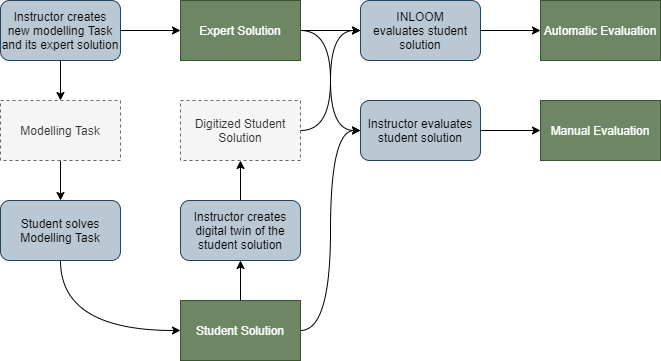
\includegraphics[size=0.8, ]{graphics/AvailableData.png}

\begin{itemize}
    \item[\textbf{RQ3.1}] The software must employ a data structure, that is able to hold
    information collected on automatic and manual evaluations and enables comparing the two.
\end{itemize}

\subsection{INLOOM Result Files}
The first part of the available data are the results produced by INLOOM. INLOOM persists its 
results in form of XML files. Each of the XML files, contains the results of the constraints 
applied to one student solution, as well as some meta data. The format used in these files,
has changed since the publication of \cite{1} and is now described by the following DTD:

\lstset{language=XML}
\begin{lstlisting}[caption={
    XML format, currently used to persist the results the INLOOM software generates.
}, captionpos=b]
<!ELEMENT TestResult (TestData, Results, ResultPoints)>

<!ELEMENT TestData (ExpertModel, TestModel)>
<!ELEMENT ExpertModel EMPTY>
<!ATTLIST ExpertModel id CDATA #REQUIRED>
<!ELEMENT TestModel EMPTY>
<!ATTLIST TestModel id CDATA #REQUIRED>
<!ELEMENT MetaModel EMPTY>
<!ATTLIST MetaModel type CDATA #REQUIRED>
<!ELEMENT MCSIdentifier EMPTY>
<!ATTLIST MCSIdentifier id CDATA #REQUIRED>
<!ELEMENT MCSVersion EMPTY>
<!ATTLIST MCSVersion value CDATA #REQUIRED>

<!ELEMENT Results (CResult+)>

<!ELEMENT CResult (
    ExpertObject, ExpertType, TestObject, TestType
    Rule, Category, Points, Msg
)>
<!ELEMENT ExpertObject (#PCDATA)>
<!ELEMENT ExpertType (#PCDATA)> 
<!ELEMENT TestObject (#PCDATA)> 
<!ELEMENT TestType (#PCDATA)>  
<!ELEMENT Rule (#PCDATA)>  
<!ELEMENT Category (#PCDATA)>  
<!ELEMENT Points (#PCDATA)>  
<!ELEMENT Msg (#PCDATA)>  

<!ELEMENT ResultPoints (MaxPoints, TestPoints)>  
<!ELEMENT MaxPoints (#PCDATA)>  
<!ELEMENT TestPoints (#PCDATA)>  
\end{lstlisting}

The root of the XML files is the "TestResult". All meta data is stored in "TestData", while
the individual constraint results are persisted as a list of "Result" under "Results".

Each such "Result" identifies the element, used during the constraint generation from the expert
solution, in "ExpertObject" and "ExpertType". The matching element of the student solution is
stored in "TestObject" and "TestType". The "Object" Part, holds the label or name of the used
element. The "Type" Part stores the type of the element in the diagram. What types INLOOM is able
to detect and grade, depends on the meta model used for the evaluation \cite{1}.

In the "TestData" branch, information about the result is available. The "id" contained in 
"ExpertModel" references the expert solution the students work was compared to. "TestModel"
identifies the evaluated student solution. "MetaModel", "MCSIdentifier" and "MCSVersion" are
contain versioning information about the created evaluation. These tags are interesting for 
making sure, that only evaluations, that were created und the same circumstances are compared.

The amount of test data sets will most probably not increase dramatically in the near future,
so there is no reason, to reduce the result data in any way before using it for testing.
This leads to 

\subsection{Manually Evaluated Student Solutions}
The second part of the test data are manual evaluations of student solutions. Thirty already
graded pen-and-paper student solutions to exam tasks were digitally reproduced by \cite{1}, to 
evaluate them using INLOOM. Of these thirty solutions, ten are solutions to exam tasks of the
summer term exams 2016, 2017 and 2018. Of the evaluations to this student solutions, only an 
analog version exists.

The manual evaluations of these digitized student solutions are the best evaluations known for
the specific solution and therefore, are the only measure of quality one can apply to INLOOM. 
It can be assumed that the automatic evaluations quality is sufficient, if it reaches the same
result as the manual evaluation. 

In order to compare these manual evaluations to the ones automatically generated by INLOOM 
however, they need to be digitized. Right now, the available manual evaluations consist of
a number of handwritten annotations in the student solutions. The annotations are mostly 
checkmarks and points awarded for elements of the model. What feature the annotation references
is indicated by its position in the student solution. Due to that format and the fact that the
student solutions were stored as black and white scans, it is unlikely that the evaluation data
can be automatically extracted. Therefor it's necessary to provide an evaluation digitization
facility.

\begin{itemize}
    \item[\textbf{RQ3.2}] The software must include a facility to digitize manually created 
    evaluations of student solutions. 
\end{itemize}

\subsection{Common Elements of Automatic and Manual Evaluations}
There are some elements automatic and manual evaluations obviously have in common. Others are
more oblique and some transformation is required, before they can be assumed present in both. 

Each of the evaluations, was made for exactly one \textit{student solution} to exactly one 
\textit{exercise}. Each evaluation can only ever be created by one \textit{evaluator} and 
using one \textit{expert solution} for reference. For testing purposes, there is no point 
in comparing an automatic evaluation to a manual one, if they differ in one of these attributes.

For one student solution, there can exist multiple automatic and manual evaluations. Multiple
manual evaluators or different version of the INLOOM software could create an evaluation for 
the same student solution. The literature research showed, that it can be interesting to inspect
multiple manual evaluations of the same student solution, created by different evaluators. Each
evaluator has his/her own style and preferences, which will be reflected in the evaluation.

\begin{itemize}
    \item[\textbf{RQ3.3}] The software must be able to persist multiple evaluations for the 
    same student solution. 
\end{itemize}

\subsection{Digitizing Manual Evaluations}
The need to digitize the manual evaluations before being able to compare them automatically
to the automatic evaluations INLOOM produces, means a huge overhead for the testing process. 